\documentclass[USenglish,twocolumn]{article}

\usepackage[utf8]{inputenc}%(only for the pdftex engine)
%\RequirePackage[no-math]{fontspec}%(only for the luatex or the xetex engine)
\usepackage[big]{dgruyter}
\usepackage{algorithm}
\usepackage{algpseudocode}
\usepackage{booktabs}
\usepackage{array}
\usepackage{subcaption}
\setlength\extrarowheight{2pt}
%MOJE!
\usepackage{xstring}
\newcommand{\Ref}[2]{%
    \IfEqCase{#1}{%
	    {fig}{Figure~\ref{#2}}%
	    {tab}{Table~\ref{#2}}%
	    {equ}{Equation~\ref{#2}}%
        % you can add more cases here as desired
    }[\PackageError{tree}{Undefined option to tree: #1}{}]%
}%
\usepackage{float}
\usepackage{gensymb}
\usepackage{bm}
\usepackage{hyperref}

\begin{document}
 
  \articletype{Research Article{\hfill}Open Access}

  \author[1]{Piotr Napieralski}

  \author[2]{Filip Rynkiewicz}

  \affil[1]{\mbox{Institute of Information Technology}, Lodz University of Technology, \mbox{e-mail: piotr.napieralski@p.lodz.pl}}

  \affil[2]{\mbox{Institute of Information Technology}, Lodz University of Technology, \mbox{e-mail: 173186@edu.p.lodz.pl}}

  \title{\huge Modeling Human Pupil Dilation to Decouple the Pupillary Light Reflex}

  \runningtitle{Modeling Human Pupil Dilation to Decouple the Pupillary Light Reflex}

  %\subtitle{...}

\begin{abstract}
\indent The aim of this paper is to present methods to calculate pupil size based on various parameters, such as: luminance, age, corneal flux density or monocular/binocular effect. These models allow to distinguish pupil dilation caused by the influence of light and other factors such as psychological state of participants.The developed methods were presented based on empirical data. Various researchers estimate their equations based on oculographic data obtained in the course of experiments. The presented plots are based on those equations. Different approaches can be compared to show the difference between particular models.The methods presented in this paper enable a more detailed investigation of the influence of various parameters on the pupil. It can be used to better estimate the influence of light on pupil size. The main changes occurring in pupil size, i.e. contractions and dilation, are caused by light. Other criteria such emotional arousal, cognitive processes or even memory operations can also alter the pupil, among which the decoupling of light is important. The presented approach is distinct from other similar studies because it decouples the pupillary light reflex.
\end{abstract}
  \keywords{pupil dilatation, pupilary light reflex, eye tracking}
  
  %\classification[PACS]{}
  %\communicated{...}
  %\dedication{...}

  \journalname{Physics}

  \DOI{DOI}
  \startpage{1}
  \received{..}
  \revised{..}
  \accepted{..}

  \journalyear{2014}
  \journalvolume{1}
  \journalissue{11}

\maketitle

\section{Introduction}

\indent The human eye is a complex biological structure, sensitive to light and pressure. Thanks to its structure, this  organ provides one of the most important senses for humans, which is vision. For million years of evolution, the mammal eye has been able to differentiate between about 10 million colors and it is possibly capable of detecting a single photon. For the purpose of this research, the anatomy of the eye human has been simplified (see \Ref{fig}{fig:anatomy}).

\begin{figure}[ht!]
	\centering
	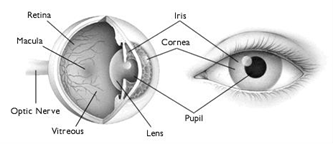
\includegraphics[width=0.48\textwidth]{img/anatomy.png}
	\caption{Anatomy of human eye \textit{https://goo.gl/k5qap4}}
	\label{fig:anatomy}
\end{figure}
\indent Light passes through the cornea, the pupil and the lens to finally fall on the light-sensitive cells of the retina. When the amount of light coming through the iris exceeds the normal requisition, or there is a shortage of light for the eye to achieve normal vision, the \textbf{iris sphincter muscle}and \textbf{iris dilator muscle} react, creating what is known as the \textit{pupillary light reflex}. The first muscle constricts the pupil when light is too bright, while the other expands it in poor light conditions. In a heightened sympathetic activity, these muscles can follow the same response pattern as in the case of various light conditions. The varying size of the pupil is a physiological response to many external factors (the pupillary response). The change in pupil size can be prompted by an involuntary reflex reaction to light (exposure to light) \cite{Saladin}. An increase in the size of the pupil of the eye has been found to accompany interest understood in the context of attention, and even sexual arousal \cite{Hess} \cite{Hammerer}. Other factors are memory operations \cite{Bradley} or a cognitive effort to distinguish between automated and controlled cognitive processing \cite{Querino} \cite{Staniucha} In normal light conditions, the pupil the pupil diameter is around 3.09mm, and 4.93mm for darkness \cite{Wyatt}. In \Ref{fig}{fig:dilatation}, the effect of bright light and dim light is presented. As far as the latency of the light reflex, the shortest one was recorded in \cite{Ellis} and it was 220 ms. Some algorithms aiming to create a virtual pupil \cite{Walraven} can be found in the literature, which can be used to conduct experiments without the need for human subjects.
\begin{figure}[H]
	\centering
	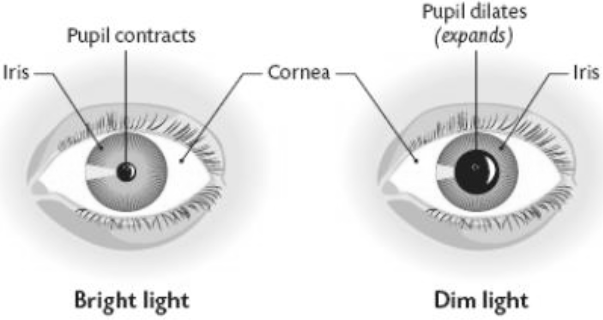
\includegraphics[width=0.48\textwidth]{img/dilatation.png}
	\caption{Pupil dilatation based on given light \cite{Walker}}
	\label{fig:dilatation}
\end{figure}
The pupillary light reflex is modeled as a physiologically-based non-linear delay differential equation. 
Subsequent pupillary measurements will be made with a different physiological index. It is observed that the pupil diameter changes each fixation cross location in the different emotional state \cite{Raiturkar}. The magnitude of the pupil is strongly correlated with visual attention and task performance \cite{Ebitz}. The numerical accuracy of different variants of integral image computation algorithms allow for the possibility of multiple evaluations of different statistical characteristics of the image \cite{Puchala} to extract the differences from different parameters of the pupil size. 
The other solution is based on artificial neural networks \cite{Garbaa} \cite{Lipinski} used to predict the pupillary response and factor localization. 
\cite{Raiturkar} propose a model based on the fact that the pupil’s response to brightness changes is linear and they try to cover the range of pupillary behavior. They assume that the response of the pupil, at each time instant, is independent of the previous light intensity that it was exposed to.
Models of pupil changes under the influence of light may allow us to separate factors related to the emotional state of the human study subject from the rate of these emotional cues. We propose to collect information about pupil dilation and then decouple the pupillary light reflex from this data. It is important to know the behavior of the eye due to changes in the light environment. Currently, studies on emotional states based on pupil size are performed in isolated laboratory environments. Accordingly, knowing and modeling pupil changes based on light conditions will allow us to isolate these changes. To ensure the most accurate simulation of pupil behavior, we implemented and the most popular mathematical models of the pupillary light reflex
 \section{Pupillary light reflex in equilibrium state}
 The pupillary light reflex is the main mechanism that regulates the pupillary diameter. Most models so far have been developed against the background of empirical research. Data gathered in those experiment was obtained after the pupil reached the equilibrium state, when the pupil stabilized for each illumination level. Those models are not suitable for describing dynamic changes of the pupil, but are used as a base for some models of dynamic changes of the pupil. The literature describes several dynamic behavior models built around experiments designed to measure the values of some parameters as a function of incident light intensity \cite{Pamplona}, described in <add reference> .
 Calculation of pupil size in am equilibrium state based on given illumination can be performed using multiple formulas, which are presented at below. 
 Based on \cite{Watson}, the entire equation was transformed to use \textbf{nit}(${cd}/{m^{-2}}$) as the main unit of luminance. 
 \\ \indent The first study was aimed at extrapolating pupil size based on given luminance was conducted by Holladay \cite{Holladay}. Data was collected for 3 participants of unknown age and binocular viewing.
 \begin{equation}
	 D_{H}(L) = 7\exp(-0.1007L^{0.4})
	 \label{equ:holladay}
 \end{equation}
\begin{figure}[H]
	\centering
	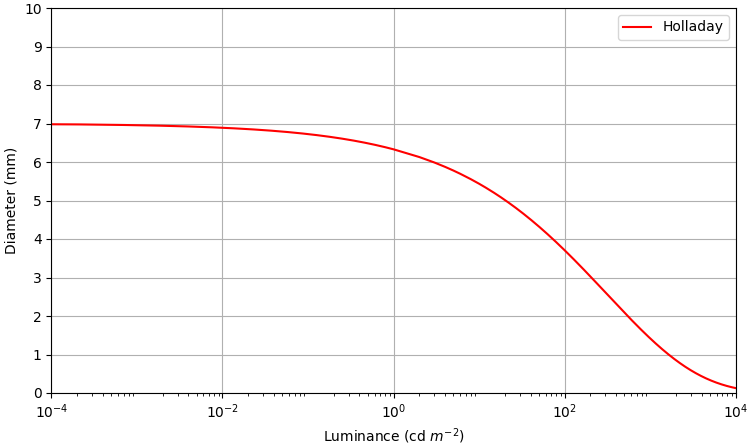
\includegraphics[width=0.48\textwidth]{img/holladay.png}
	\caption{Pupil size for \protect\Ref{equ}{equ:holladay} of Holladay}
	\label{fig:holladay}	
\end{figure}

 \begin{equation}
	 D_{C}(L) = 5 - \tanh[0.61151 + 0.447\log L]
	 \label{equ:crawford}
 \end{equation}
 \begin{figure}[H]
	\centering
	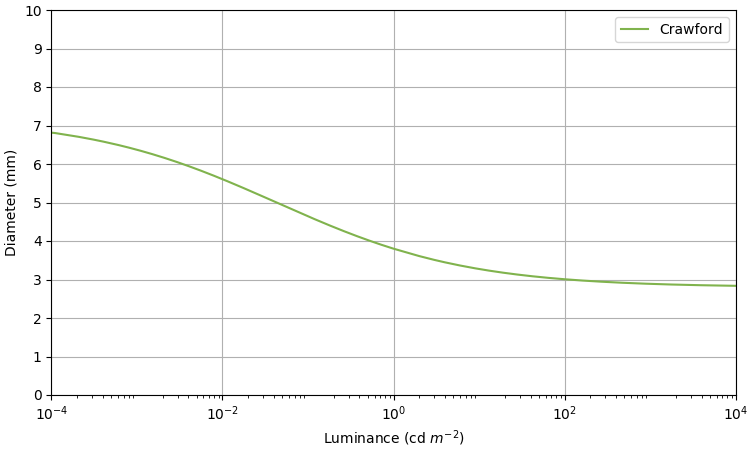
\includegraphics[width=0.48\textwidth]{img/crawford.png}
	\caption{Pupil size for \protect\Ref{equ}{equ:crawford} of Crawford}
	\label{fig:crawford}
\end{figure}
\Ref{equ}{equ:holladay} plotted at \Ref{fig}{fig:holladay} fails for high luminance beyond $\approx 600cd/m^{-2}$ for 2mm asymptote. As in the previous study, a study by Crawford \cite{Crawford} also fails to reveal the age of its subjects, but their adapting field diameter is 55\textdegree. In this examination, the author took samples from 10 people. It can be observed that the asymptote of 2mm given in Holladay is not present (see \Ref{fig}{fig:crawford}). Moon and Spencer \cite{Moon}, based on the equation and data approximation provided by Crawford, Blanchard \cite{Blanchard} and Reeves \cite{Reeves}, developed a slightly different formula, plotted in \Ref{fig}{fig:moonSpancer}.
\begin{equation}
	D_{MS}(L) = 4.9 - 3\tanh[0.4\log L]
	\label{equ:moonSpancer}
\end{equation}
 \begin{figure}[H]
	\centering
	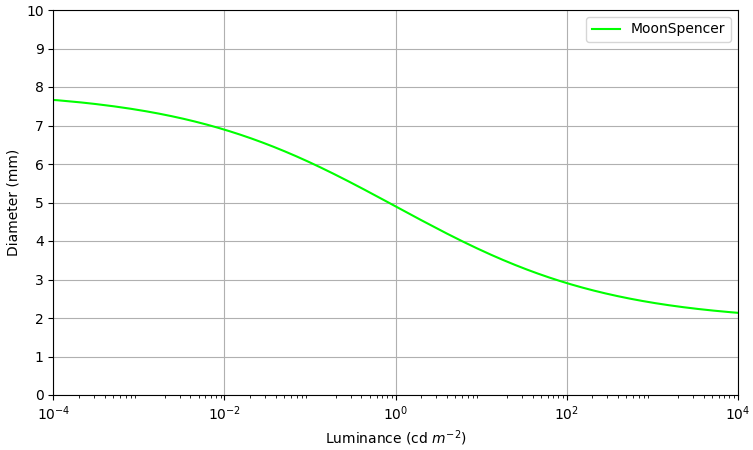
\includegraphics[width=0.48\textwidth]{img/moonSpancer.png}
	\caption{Pupil size for \protect\Ref{equ}{equ:moonSpancer} of Moon and Spencer}
	\label{fig:moonSpancer}
\end{figure}
De Groot and Gebhard \cite{de_Groot} formulated an equation based on the averaged data from previous work, taking into consideration the number of people examined in the experiment. As can be seen in \Ref{fig}{fig:groot}, the asymptote of 2mm is not present in this formula either. According to the authors, it is not necessarily demanded by the data of the physiological restrictions.

\begin{equation}
   D_{DG}(L) = 7.175 \exp [-0.00092(7.597 + \log L)^{3}]
	\label{equ:groot}
\end{equation}
 \begin{figure}[H]
	\centering
	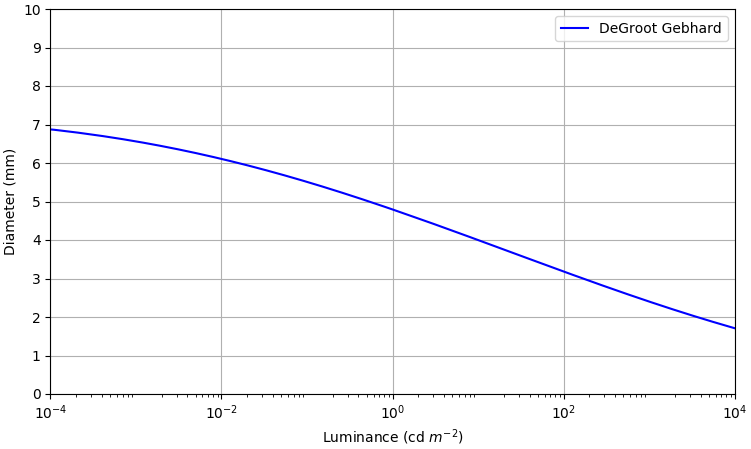
\includegraphics[width=0.48\textwidth]{img/groot.png}
	\caption{Pupil size for \protect\Ref{equ}{equ:groot} of De Groot and Gebhard}
	\label{fig:groot}
\end{figure}

Important changes in the formulas were introduced by Stanley and Davies \cite{Stanley}. In contrast to previous work which assumed that dilatation depend only on a given luminance, they went on to conclude, based on Crawford, that the pupil diameter is directly correlated with the product of luminance \textit{L} and the \textit{adapting field size}, expressed by a in $deq^2$, which gives \textit{corneal flux density}($cdm^-2 deq^2$). To arrive at this formula, data was gathered from 6 volunteers whose adapting field size ranged from 0.4\textdegree  to 25.4\textdegree. These two values were plotted at \Ref{fig}{fig:stanleyDavies} and used as thresholds for this experiment.
\begin{equation}
	D_{SD}(L, a) = 7.75 - 5.759 \frac{(La/846)^{0.41}}{(La/846)^{0.41} + 2}
	\label{equ:stanleyDavies}
\end{equation}
 \begin{figure}[H]
	\centering
	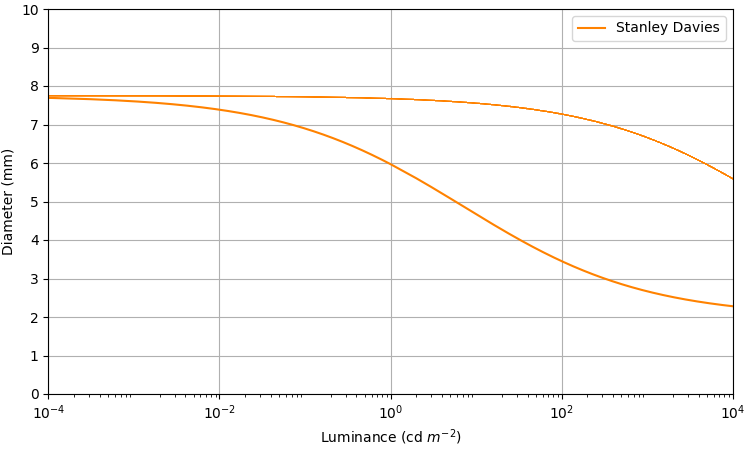
\includegraphics[width=0.48\textwidth]{img/stanleyDavies.png}
	\caption{Pupil size for \protect\Ref{equ}{equ:stanleyDavies} of Stanley and Davies. Field diameter 0.4\textdegree(first line) and 25.4\textdegree(second line) }
	\label{fig:stanleyDavies}
\end{figure}
Barten \cite{Barten} developed his own formula based on Moon and Spencer and Stanley Davies consideration of field size.
\begin{equation}
	D_{SD}(L, a) = 5 - 3\tanh(0.4\log \frac{La}{40^{2}})
	\label{equ:barten}
\end{equation}
 \begin{figure}[H]
	\centering
	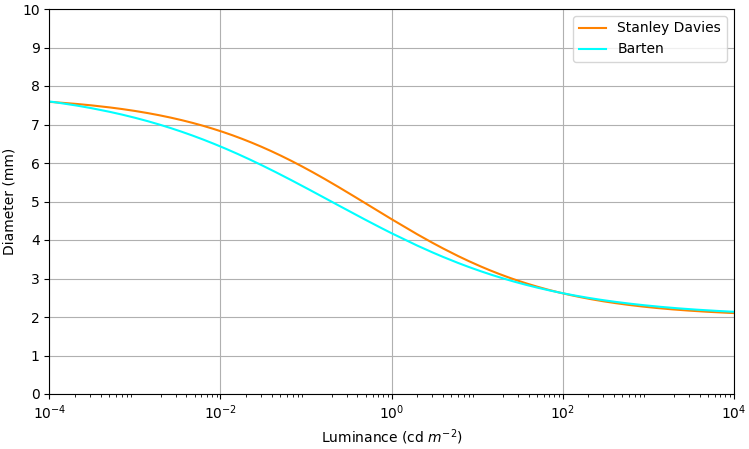
\includegraphics[width=0.48\textwidth]{img/barten.png}
	\caption{Pupil size for \protect\Ref{equ}{equ:barten} Barten plotted against Stanley and Davies.}	
	\label{fig:barten}
\end{figure}
Blackie and Howland \cite{Blackie}, based on a big project of modeling the emmetropization experiment, designed a formula expressed by:
\begin{equation}
D_{BH}(L) = 5.697 -0.658 \log L - 0.07(\log L)^{2}
\label{equ:blackieHowland}
\end{equation}
\begin{figure}[H]
	\centering
	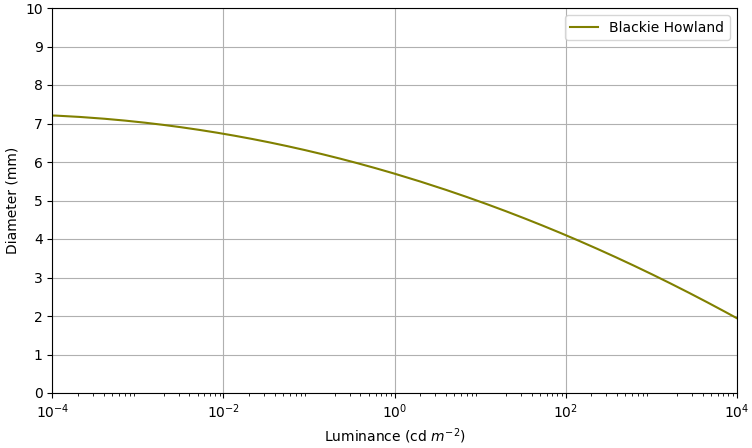
\includegraphics[width=0.48\textwidth]{img/blackieHowland.png}
	\caption{Pupil size for \protect\Ref{equ}{equ:blackieHowland} Blackie and Howland.}	
	\label{fig:blackieHowland}
\end{figure}
\cite{Winn} Winn carried out an experiment for 91 subjects aged from 17 to 83, including students, staff and the clinical population of Aston University. Subjects maintained a steady fixation at the center of an evenly illuminated circular field with a 10\textdegree diameter. Pupil diameter was measured at five luminance levels (9, 44, 220, 1100, and 4400 $cdm^{-2}$ ). The mean pupil size of 91 subjects was plotted as a function of age for five different levels of luminance. Thanks to this data, the slope and intercept were estimated. These values are given in \Ref{tab}{tab:winn}.
\begin{table}[H]
	\centering
	\caption{Estimated slopes and intercept for Winn etc.}
	\label{tab:winn}
	\begin{tabular}{|l|l|l|l|}
		cd \bm{$m^{-2}$ } &  slope & intercept &\bm{$r^2$}\\ \midrule
		9 & -0.043 & 8.046 &0.0557\\ \hline 
		44	&-0.04&	7.413&	0.0486\\ \hline
		220	&-0.032&	6.275&	0.377\\ \hline
		1100&	-0.02&	4.854&	0.0226\\ \hline
		4400&	-0.015&	4.07&	0.214 \\
	\end{tabular}
\end{table}
Luminance was restricted to illumination in Winn et al.’s experiment. To use values from \Ref{tab}{tab:winn} in pupil prediction equation, the slope needs to be presented as a function of log luminance with a cubic polynomial (see \Ref{equ}{equ:winnPoly}). The same pattern was followed in the case of the intercept (see  \Ref{equ}{equ:winnIntercept}).
\noindent
\begin{equation}
\label{equ:winnPoly}
\begin{split}
	&W_{s}(L) = \sum_{k=0}^{3} S_{K}\left(  \log \left(\min\left(4400,\max \left(9,L\right)\right)\right)\right)^{k} \\
	&s_{0}= -0.24501\\
	&s_{1}= -0.0368073\\
	&s_{2}= 0.210892\\
	&s_{3}= 0.00281557
\end{split}	
\end{equation}
\begin{equation}
\label{equ:winnIntercept}
\begin{split}
&W_{I}(L) = \sum_{k=0}^{3} b_{K}\left(  \log \left(\min\left(4400,\max \left(9,L\right)\right)\right)\right)^{k} \\
&b_{0}= 6.9039\\
&b_{1}= 2.7765\\
&b_{2}= -1.909\\
&b_{3}= 0.25599
\end{split}	
\end{equation}
hen, to estimate the data of Winn et al.., both functions were combined:
\begin{equation}
\label{equ:winn}
D_{W}(L,y) = W_{S}(L)y + W_{I}(L)
\end{equation}
where $y$ denotes the age of a participant.
\begin{figure}[H]
	\centering
	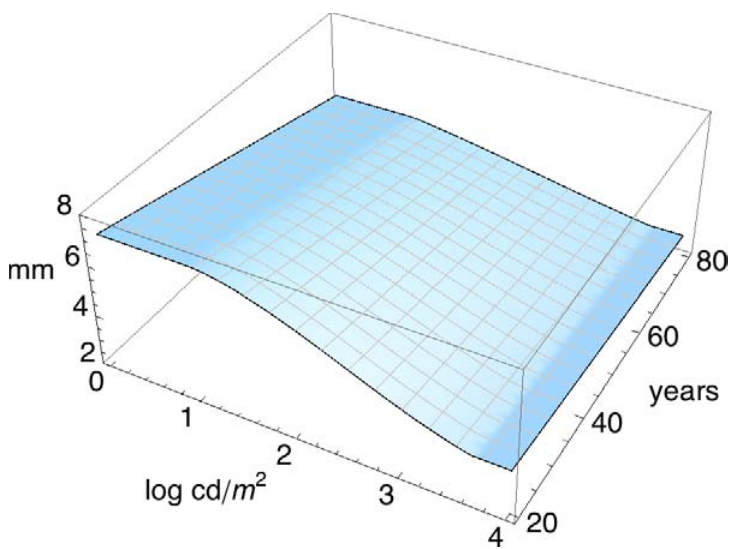
\includegraphics[width=0.48\textwidth]{img/winn.png}
	\caption{Pupil size for \protect\Ref{equ}{equ:winn} off Winn.}	
	\label{fig:winn}
\end{figure}

Wattson and Yellot \cite{Watson} created unified formula, which combines the previously described equation as well as considering new parameters.

Taking into account previously conducted experiments in which only the dilatation of one eye was measured where the result differs from the experiments with both, given in the same adapting light (as in the \Ref{fig}{fig:bin_mon}), the monocular effect was created. Based on a comparison of mono and binocular data the conclusion was that the modeling of the monocular effect can be superimposed by a horizontal shift on a log axis. In which the average optimal shift of monocular data to match binocular data amounted to 0.1015. With this information, a the factor of 0.1 can be used to shift data when in an experiment only one eye is examined, and 1 when the data is collected on the binocular (\Ref{equ}{equ:WattsonYellot_Bin})
\begin{equation}
\label{equ:WattsonYellot_Bin}
\begin{split}
&M(1) = 0.1 \\
&M(2) = 1
\end{split}	
\end{equation}
In addition to using the monocular effect, the \textit{effective corneal flux density} formula was also developed, which extends the previous corneal flux density by:
\begin{equation}
\label{equ:WattsonYellot_ecfd}
F = LaM(e)
\end{equation}
The result is the product of luminance, adapting area and monocular effect.
\begin{figure}[H]
	\centering
	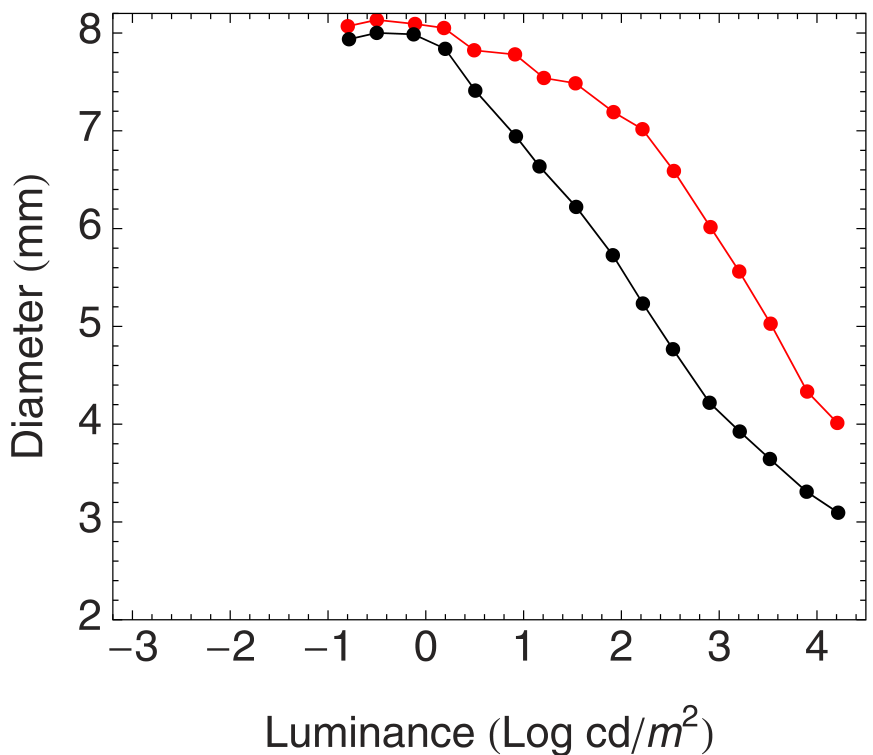
\includegraphics[width=0.30\textwidth]{img/bin_mon.png}
	\caption{Binocular and monocular data from Doesschate and Alpem \cite{Doesschate}}	
	\label{fig:bin_mon}
\end{figure}
In Winn et al. the age of participant was given as a crucial parameter in pupil size approximation, although data was limited to 4400 $cdm^{2}$ and the adapting field size of 10\textdegree. Assuming a linear relation between the slope function from Winn et al. and the pupil diameter calculated in Stanley Davies for the same luminance, the new general slope function could be designed.
\begin{equation}
\label{equ:WattsonYellot_slope}
S(L,a,e)=0.02132-0.0095623D_{SD}(LM(e),a)
\end{equation}
The rate of change of the pupil diameter with age was estimated based on the function of luminance, area flux density, age, referenced age and eye function.
\begin{equation}
\label{equ:WattsonYellot_A}
\begin{split}
&A(L,a,y,y_0,e)=(y-y_0 )S(L,a,e), \\
&20 \leq y \leq 83
\end{split}	
\end{equation}
Age must be in the range of that of the subjects in Winn et al. Reference age is the age of observers in the experiment. As far as reference age in the equation of Wattson Yellot, it is equal to 28.58, which is the average age of the subjects in the Stanley Davies study.
\begin{figure}[H]
	\centering
	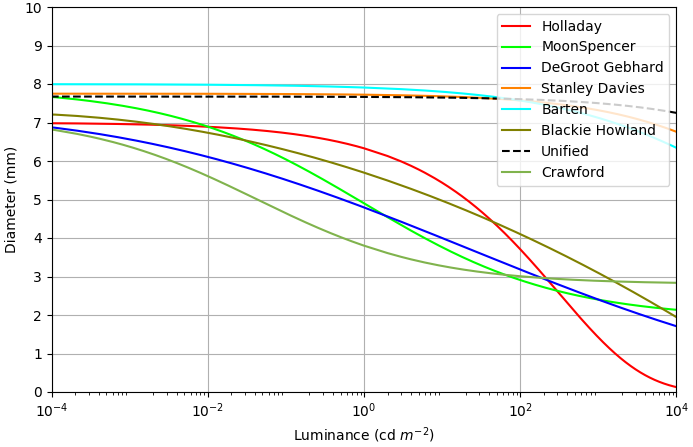
\includegraphics[width=0.48\textwidth]{img/wattsonYellot_1.png}
	\caption{Pupil size for \protect\Ref{equ}{equ:WattsonYellot_A} of Watson and Yellot, compared to all previous models.\ a=10°, monocular.}	
	\label{fig:wattsonYellot_1}
\end{figure}
\begin{figure}[H]
	\centering
	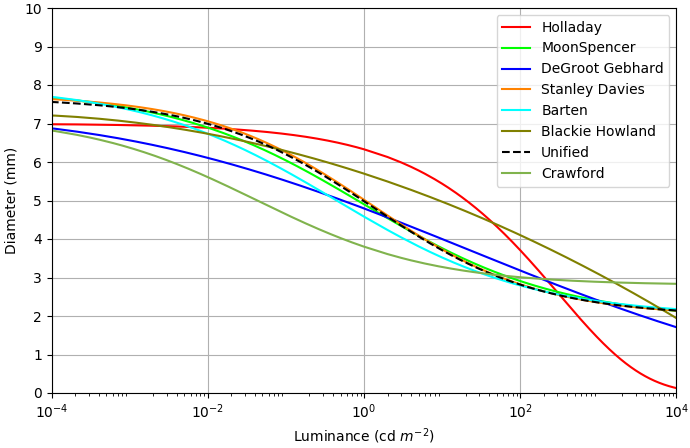
\includegraphics[width=0.48\textwidth]{img/wattsonYellot_2.png}
	\caption{Pupil size for \protect\Ref{equ}{equ:WattsonYellot_A} of Watson and Yellot, compared to all previous models.\ a=60°, binocular.}	
	\label{fig:wattsonYellot_2}
\end{figure}
\Ref{fig}{fig:wattsonYellot_1} and~\ref{fig:wattsonYellot_2} show all the described methods and they demonstrate that these methods can differ depending on the parameters. \Ref{fig}{fig:wattsonYellot_1} presents monocular e=2 data from a small adapting area a=10. It can be seen that the Unified formula, based on Stanley and Davies, gives similar results to the Barten formula. Meanwhile In \Ref{fig}{fig:wattsonYellot_2}, it can be observed that the Unified, Barten, Stanley Davies and Moon-Spencer formulas give similar results, which shows that the Watson and Yellot model can be used to predict pupil size more precisely than previous models
\section{Dynamic model of pupillary light reflex}
As described in previous chapter, models only give information about pupil size after adaptation to a given light luminosity. Meaning that it does not describe changes of the pupil in a time interval. This poses a significant problem in research which includes constant changes of light or in monitoring the changes on psychological impulses. Models of such changes need to take into consideration the specific physiological behavior of the pupil.
In the case of PLR, iridial reaction is caused by light striking through the retina. This action sends a neural signal, but it needs time to cause the iridial reaction, which is why it is modelled by a time delayed equation. Another parameter that affects the pupil change is the threshold value of light flux. Luminosity higher than that given threshold will not cause the pupil to react. 
As the final visual effect of PLR is the movement of dilator and sphincter muscles, there are PLR models that are designed to simulate behavior of those muscles based on autonomic nervous system input. In \cite{Fan} the model is targeted to simulate only short light flashes, which does not cover all possible cases of PLR behavior. The model presented at \cite{Suaste-Gomez} is over complicated with multiple second-order delay differential equations, and thus it is impractical for designing a robust inverse algorithm to obtain model parameters from experimental data.
The model used in this experiment is based on the Moon and Spencer equation\ref{equ:moonSpancer}, for equilibrium pupil state, and Longtin and Milton’s time dependent pupil size which is described by a time delayed equation. The \Ref{equ}{equ:Pampelona} describes the behavior of dynamic changes of the pupil in response to light where the pupillary latency – the time delay between the instant in which the light pulse reaches the retina and the beginning of iridial reaction – is given by $\tau$ and time \textit{t}. Parameter \textit{D} describes the pupil diameter in millimeters, which is the output of the solved equation.  
This model is able to describe changes of the individual pupil in specific light conditions. Despite the fact that Pamplona is based on Moon and Spencer’s function and not the newest Wattson and Yellot, the literature shows that this method gives very high correlation with real life scenarios.

\begin{equation}
\label{equ:Pampelona}
\frac { d M } { d D } \frac { d D } { d t } + 2.3026 \operatorname { atanh } \left( \frac { D - 4.9 } { 3 } \right) = 5.2 - 0.45 \ln \left[ \frac { \phi ( t - \tau ) } { \overline { \phi } } \right]
\end{equation}

\section{Description of the research environment}
In order to record pupil changes caused by either internal or external factors, a device called an eye-tracker can be used. The main task of this device is to track and record gaze, but in addition, vital oculography parameters can be recorded. Blink occurrence frequency, saccades detection and real time pupil size monitoring, are the most common ones. In order to record those changes multiple cameras, either InfraRed or RGB, must be used. The arrangement of those cameras can be used to distinguish two main types of eye trackers. 

Head-mounted eye trackers, mostly in the shape of glasses, have multiple cameras aimed directly onto the subject’s eyes, and one so-called global camera to record the scene in front of the subject.  The greatest advantage of these devices is their mobility, which allows the subject to move their head freely and change locations. The biggest disadvantage is that they have lower precision and accuracy compared with stationary ones, because of the subject’s head movement.

The second type of eye-trackers are so-called remote-eye trackers. This is a nonintrusive peripheral device that has no contact with human body. Cameras that are placed inside this device are aimed in front of the scene, where the face of subject must be present. These are stationary devices with no possibility of changing its location, thus the test must take place in same area. The biggest advantage over the wearable eye tracker is that this kind of eye tracker is nonintrusive, which is more suitable to study psychological reflexes. Thus, the device is calibrated in a way that has a certain window where the eye of the subject must be visible and there is no head movement of subject. Accuracy is higher in comparison with a wearable one.

Taking into consideration that experiment is aimed at real life scenarios like shopping, walking in the street, or sport event activity, the most important property of the device must be its mobility. Based on other research and solutions available on the market, the wearable eye tracker was chosen for this experiment. The second attribute of the device must be the possibility to develop and implement new algorithms for measuring pupil changes over time. There are multiple DYI wearable eye-trackers, but they lack precision and accuracy in comparison to devices provided by commercial solutions. Based on devices available for our use, the Tobii Pro Glasses 2, and Pupil Lab \Ref{fig}{fig:pupilLab_e}, both were tested in accuracy and precision. The conclusion of the preliminary conducted experiment was that the Tobii Pro Glasses 2 have slightly better results than the other device. The lack of possibility to extend usage of Tobii by adding new algorithms or another peripheral device resulted in the Pupil Lab being chosen as the best choice.

This device is capable of gaze estimation with 0.6 degree of visual angle (0.08 degree precision) with a processing pipeline latency of only 0.045 seconds, blink detection, pupil size monitoring and more. The glasses-like headset eye tracker, presented at Figure 14, consists of two RGB cameras with an IR filter and one global directed RGB camera at the front of the user. The frontal camera is able to capture an image at a max resolution of 1920x1080 pixels at 30Hz with a 90-degree diagonal field of view. Two IR cameras, which can operate up to 200Hz, are located at glasses frames and aimed directly at the eyes of the subject. 
Software used in Pupil Lab uses the “dark pupil” detection method,presented at \Ref{fig}{fig:pupilLab}, thus, IR cameras must be able to capture video at a specific range of the IR spectrum, in this device it is a 860nm wavelength.  Each image captured by the IR camera is analyzed by open source Pupil Lab software. Thanks to the flexibility and extensibility of the source code, additional sensors can be added to this eye tracker. Additionally, in the case of this research, a simple luxometer was added to eye tracker as an external sensor.  
The BH1603FVC Rohm\footnote{\url{http://rohmfs.rohm.com/en/products/databook/datasheet/ic/sensor/light/bh1603fvc-e.pdf}} \Ref{fig}{fig:luxometer} analog current output ambient light sensor was used to determine the amount of light cast at the pupil. It is a device with a compacted surface of 3.0 x 1.6 mm and a spectral sensitivity close to human eye sensitivity.  The sensor is capable of measuring ambient light in a range of 0 - 1 000 lux on H-Gain Mode, 0 – 10 000 in M-Gain and 0 – 100 000 on L-Gain.  To measure which range will be most suitable for the conducted experiment the sensor was placed with 50cm range from LED lamp. This experiment gave values from 6 000 to 9 000 lux, which remains in the H-Gain range of the sensor and in that mode the sensor was calibrated. This sensor was placed near the IR camera of the left eye, and only these eye responses are recorded during the experiment.
\begin{figure}[H]
	\captionsetup[subfigure]{justification=centering}
	\centering
	\begin{subfigure}[b]{0.3\textwidth}
		\centering
		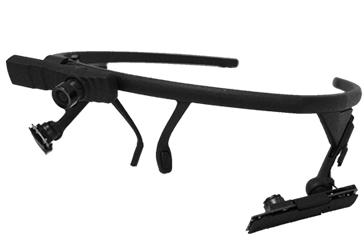
\includegraphics[width=0.9\textwidth]{img/pupilLab.png}
		\caption{Pupil Lab eye tracker}
		\label{fig:pupilLab_e}
	\end{subfigure}
	~ %add desired spacing between images, e. g. ~, \quad, \qquad, \hfill etc. 
	%(or a blank line to force the subfigure onto a new line)
	\begin{subfigure}[b]{0.5\textwidth}
		\centering
		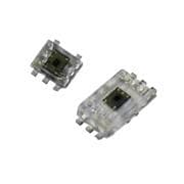
\includegraphics[width=0.3\textwidth]{img/rohm.png}
		\caption{BH1603FVC Rohm sensor}
		\label{fig:luxometer}
	\end{subfigure}
	\caption{Pupil Lab eye tracker and BH1603FVC Rohm sensor. Source https://bit.ly/2TH3hby https://bit.ly/2VbrV1d}	
	\label{fig:sensors}
\end{figure}
To recognize and measure the changes of the pupil over time, the Pupil Lab method was used, as a default for the hardware. The detection method used in the software provided by Pupil Lab consists of 7 steps, presented at \Ref{fig}{fig:pupilLab}. First the image of eye is converted to grayscale. Using a Haar-like feature, the region of interest – the estimated region where pupil can be – is calculated, and significantly cut the unwanted pixels from source image (\Ref{fig}{fig:pupilLab1}). The region obtained in the previous step is filtered by a Canny edge detector (\Ref{fig}{fig:pupilLab2}). For the region of interest, the histogram is calculated (\Ref{fig}{fig:pupilLab3}), and  the “dark” region is defined by the offset from the lowest spike in the histogram. All edges with spectral reflections and not in the “dark” region are excluded(\Ref{fig}{fig:pupilLab4}). Remaining edges are filtered and split into sub contours, based on the criteria of curvature continuity (\Ref{fig}{fig:pupilLab5}). Finally, the ellipse is fitted using the least square method and additional criteria like ellipse circumference (\Ref{fig}{fig:pupilLab6}).
\begin{figure}[H]
	\captionsetup[subfigure]{justification=centering}
	\centering
	\begin{subfigure}[b]{0.15\textwidth}
		\centering
		\includegraphics[width=0.9\textwidth]{img/PupilLab/1.png}
		\caption{}
		\label{fig:pupilLab1}
	\end{subfigure}%
	\begin{subfigure}[b]{0.15\textwidth}
		\centering
		\includegraphics[width=0.9\textwidth]{img/PupilLab/2.png}
		\caption{}
		\label{fig:pupilLab2}
	\end{subfigure}%
	\begin{subfigure}[b]{0.15\textwidth}
	\centering
	\includegraphics[width=0.9\textwidth]{img/PupilLab/3.png}
	\caption{}
	\label{fig:pupilLab3}
\end{subfigure}

	\begin{subfigure}[b]{0.15\textwidth}
	\centering
	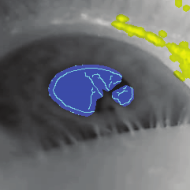
\includegraphics[width=0.9\textwidth]{img/PupilLab/4.png}
	\caption{}
	\label{fig:pupilLab4}
\end{subfigure}%
\begin{subfigure}[b]{0.15\textwidth}
	\centering
	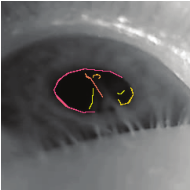
\includegraphics[width=0.9\textwidth]{img/PupilLab/5.png}
	\caption{}
	\label{fig:pupilLab5}
\end{subfigure}%
\begin{subfigure}[b]{0.15\textwidth}
	\centering
	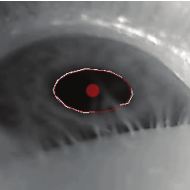
\includegraphics[width=0.9\textwidth]{img/PupilLab/6.png}
	\caption{}
	\label{fig:pupilLab6}
\end{subfigure}
	\caption{Pupil recognition algorithm in PupilLab device.}	
	\label{fig:pupilLab}
\end{figure}

\section{Experiment}
In the experiment, various scenarios were tested. In each of them, the person on whom the experiment is carried out was asked to always look forward, with the freedom to move their head, without squinting eyes to ensure that both th eye-tracker and light detector will give the best results. The figures presented below show the deviation that can be treated as non-light triggered changes. Data from luxometer and eye-tracker gathered along the experiment was used to generate the artificial signal using \ref{equ:Pampelona}\cite{Pamplona}. The real data was plotted against the generated one to find how much those two signals differ at, example at \ref{fig:experiment}. All difference is treated as pupil change caused by non-light factors, such as emotion, accommodation, etc. 

\begin{figure}[H]
	\captionsetup[subfigure]{justification=centering}
	\centering
	\begin{subfigure}[b]{0.45\textwidth}
		\centering
		%\includegraphics[width=0.9\textwidth]{img/Experiment/1.png}
			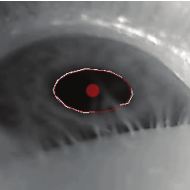
\includegraphics[width=0.9\textwidth]{img/PupilLab/6.png}
		\caption{}
		\label{fig:experiment1}
	\end{subfigure}

	\begin{subfigure}[b]{0.45\textwidth}
		\centering
		%\includegraphics[width=0.9\textwidth]{img/Experiment/2.png}
			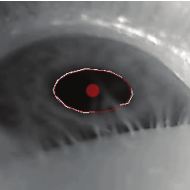
\includegraphics[width=0.9\textwidth]{img/PupilLab/6.png}
		\caption{}
		\label{fig:experiment2}
	\end{subfigure}

	\begin{subfigure}[b]{0.45\textwidth}
		\centering
		%\includegraphics[width=0.9\textwidth]{img/Experiment/3.png}
			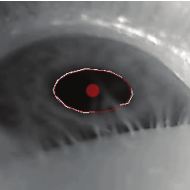
\includegraphics[width=0.9\textwidth]{img/PupilLab/6.png}
		\caption{}
		\label{fig:experiment3}
	\end{subfigure}
	\caption{Plot of data generated by \cite{Pamplona}, and data gathered by PupilLab  .}	
	\label{fig:experiment}
\end{figure}
\section{Comparison of data and model}
In \cite{Morelli} the cross-correlation technique has been shown as one possible way to compare data gathered in the conducted experiment and the modelled one. Described in the \Ref{equ}{equ:xcorr}, where  x[n] is the n point on the gathered real life data, and y[n] is the artificial generated signal. This equation returns values in rage -1 to 1, where 1 means that signals are the same, and -1 where signals are opposite.
\begin{equation}
\operatorname{norm}_{-} \operatorname{corr}(x, y)=\frac{\sum_{n=0}^{n-1} x[n] * y[n]}{\sqrt{\sum_{n=0}^{n-1} x[n]^{2} * \sum_{n=0}^{n-1} y[n]^{2}}}
\label{equ:xcorr}
\end{equation}
\begin{figure}[H]
	\captionsetup[subfigure]{justification=centering}
	\centering
	\begin{subfigure}[b]{0.45\textwidth}
		\centering
		%\includegraphics[width=0.9\textwidth]{img/Experiment/1.png}
		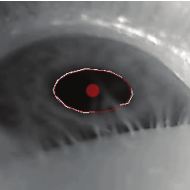
\includegraphics[width=0.9\textwidth]{img/PupilLab/6.png}
		\caption{}
		\label{fig:crossCorrelation1}
	\end{subfigure}
	
	\begin{subfigure}[b]{0.45\textwidth}
		\centering
		%\includegraphics[width=0.9\textwidth]{img/Experiment/2.png}
		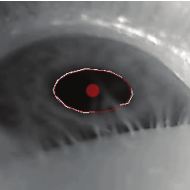
\includegraphics[width=0.9\textwidth]{img/PupilLab/6.png}
		\caption{}
		\label{fig:crossCorrelation2}
	\end{subfigure}
	
	\begin{subfigure}[b]{0.45\textwidth}
		\centering
		%\includegraphics[width=0.9\textwidth]{img/Experiment/3.png}
		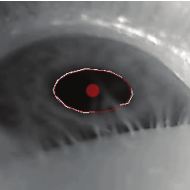
\includegraphics[width=0.9\textwidth]{img/PupilLab/6.png}
		\caption{}
		\label{fig:crossCorrelation3}
	\end{subfigure}
	\caption{Cross correlation between data gathered by devices and the artificial one.}	
	\label{fig:crossCorrelation}
\end{figure}


\section{Conclusion}
Based on the existing models, the method for measuring a light-adapted pupil diameter was implemented. We propose a solution to predict pupil size changes under visible light stimuli. The change in pupil size under the influence of light has been modeled and tested against the existing popular models. 
Subsequent pupillary measurements will be made with a different physiological index. We observed that the pupil diameter changes each fixation cross location in the different emotional state \cite{Raiturkar}. The magnitude of the pupil is strongly correlated with visual attention and task performance \cite{Ebitz}. The numerical accuracy of different variants of integral image computation algorithms allow for the possibility of multiple evaluations of different statistical characteristics of the image \cite{Puchala} to extract the differences from different parameters of the pupil size. 
The other solution is based on artificial neural networks \cite{Garbaa} \cite{Lipinski} used to predict the pupillary response and factor localization. We have adopted this solution due to its simplicity and generality. The results produced by our models are in agreement with observed behavior in humans and can be used in the eye-gaze tracking method in point of interest and attention estimation
We believe that this work can contribute to investigations of human emotion by Human Pupil Dilation. Our results should find applicability in several areas requiring eye-tracking systems, as well as in biofeedback systems. 

Scripts \url{https://github.com/MenosGrandes/PupilDiameter}, available freely and open-source
\begin{thebibliography}{99}
\bibitem{Saladin}Saladin K.,  Anatomy and physiology. New York: McGraw-Hill, 2012
\bibitem{Hess}Hess E., and Polt J.,  Pupil Size as Related to Interest Value of Visual Stimuli. Science, 132(3423), pp.349-350, 1960
\bibitem{Hammerer}Hammerer D., Hopkins A., Betts M., Maaß A., Dolan R. and Düzel E. Emotional arousal and recognition memory are differentially reflected in pupil diameter responses during emotional memory for negative events in younger and older adults. Neurobiology of Aging, 58, pp.129-139, 2017
\bibitem{Bradley}Bradley M., Miccoli L., Escrig M. and Lang P. The pupil as a measure of emotional arousal and autonomic activation. Psychophysiology, 45(4), pp.602-607, 2008
\bibitem{Querino}Querino E., dos Santos L., Ginani G., Nicolau E., Miranda D., Romano-Silva M. and Malloy-Diniz L. Cognitive effort and pupil dilation in controlled and automatic processes. Translational Neuroscience, 6(1),2015
\bibitem{Staniucha}Staniucha R, Wojciechowski A. Mouth features extraction for emotion classification, 2016
\bibitem{Wyatt}Wyatt H. The form of the human pupil. Vision Research, 35(14), pp.2021-2036, 1995
\bibitem{Ellis}Ellis C. The pupillary light reflex in normal subjects. British Journal of Ophthalmology, 65(11), pp.754-759, 1981
\bibitem{Walker}Walker H., Hall W. and Hurst J. (1990). Clinical methods. Boston: Butterworths.
\bibitem{Pamplona}Pamplona V., Oliveira M. and Baranoski G. (2009). Photorealistic models for pupil light reflex and iridal pattern deformation. ACM Transactions on Graphics, 28(4), pp.1-12.
\bibitem{Holladay}Holladay L. The Fundamentals of Glare and Visibility. Journal of the Optical Society of America, 12(4), p.271, 1926
\bibitem{Crawford}Crawford B. The Dependence of Pupil Size upon External Light Stimulus under Static and Variable Conditions. Proceedings of the Royal Society B: Biological Sciences, 121(823), pp.376-395, 1936
\bibitem{Stanley}Stanley P. and Davies A. The effect of field of view size on steady-state pupil diameter. Ophthalmic and Physiological Optics, 15(6), pp.601-603, 1995
\bibitem{Walraven}Walraven P. The virtual pupil. Journal of Modern Optics, 56(20), pp.2251-2253, 2009
\bibitem{Watson}Watson A. and Yellott J. A unified formula for light-adapted pupil size. Journal of Vision, 12(10), pp.12-12, 2012
\bibitem{Raiturkar}Raiturkar P., Kleinsmith  A., Keil A., Banerjee A., and Jain E. Decoupling light reflex from pupillary dilation to measure emotional arousal in videos. SAP '16) ACM, New York, NY, USA, 89-96,  2016
\bibitem{Garbaa}Garbaa H., Jackowska-Strumillo L., Grudzien  K., Romanowski A., (2014) Neural network approach to ECT inverse problem solving for estimation of gravitational solids flow Computer Science and Information Systems (FedCSIS),
\bibitem{Lipinski}Lipinski P. (2011). Watermarking software in practical applications. Bulletin of the Polish Academy of Sciences: Technical Sciences, 59(1).
\bibitem{Moon}Moon P. and Spencer, D. (1944). The Transient Stiles-Crawford Effect. Journal of the Optical Society of America, 34(12), p.744.
\bibitem{de_Groot}de Groot S. and Gebhard, J. (1952). Pupil Size as Determined by Adapting Luminance*. Journal of the Optical Society of America, 42(7), p.492.
\bibitem{Barten}Barten P. (2000). Contrast Sensitivity of the Human Eye and Its Effects on Image Quality. Bellingham: SPIE.
\bibitem{Blackie}Blackie C. and Howland H. (1999). An extension of an accommodation and convergence model of emmetropization to include the effects of illumination intensity. Ophthalmic and Physiological Optics, 19(2), pp.112-125.
\bibitem{Winn}Winn B., Whitaker D., Elliott D.B., and Phillips N. (1994). Factors affecting light-adapted pupil size in normal human subjects. Investigative ophthalmology \& visual science, 35 3, 1132-7.
\bibitem{Doesschate}Doesschate J., and Alpern M. (1967). Effect of photoexcitation of the two retinas on pupil size. Journal of Neurophysiology, 30(3), 562–576.
\bibitem{Blanchard}Blanchard J. (1918). The Brightness Sensibility of the Retina. Physical Review, 11(2), pp.81-99.
\bibitem{Reeves}Reeves P. (1918). Rate of pupillary dilation and contraction. Psychological Review, 25(4), pp.330-340.
\bibitem{Puchala}Puchala D., Stokfiszewski K., Numerical Accuracy of Integral Images
\bibitem{Ebitz}Ebitz, R., Pearson, J. and Platt, M. (2014). Pupil size and social vigilance in rhesus macaques. Frontiers in Neuroscience, 8.
Computation Algorithms, IET Image Processing, vol. 12, no. 1, pp. 31-41,
\bibitem{Fan}Fan, X., Yao, G. (2011). Modeling Transient Pupillary Light Reflex Induced by a Short Light Flash. IEEE Transactions on Biomedical Engineering, 58, 36-42.
\bibitem{Suaste-Gomez}Suaste-Gómez, E., Reyes Cruz, H. (2011). Inverse dynamic model of the pupil muscle plant in the simulation of response to sound, stimuli and hippus. WIT Transactions on Biomedicine and Health. 15. 407-414. 10.2495/EHR110351. 
\bibitem{Morelli}Morelli, M. S., Giannoni, A., Passino, C., Landini, L., Emdin, M., Vanello, N. (2016). A Cross-Correlational Analysis between Electroencephalographic and End-Tidal Carbon Dioxide Signals: Methodological Issues in the Presence of Missing Data and Real Data Results. Sensors (Basel, Switzerland), 16(11), 1828. doi:10.3390/s16111828
\end{thebibliography}
\end{document}
